\rfcnumber{0010}
\rfctitle{Automatic path discovery}
\rfcdate{October 2025}
\rfcauthor{@Teebor-Choka}
\section{RFC-0010: Automatic path
discovery}\label{rfc-0010-automatic-path-discovery}

\begin{itemize}
\tightlist
\item
  \textbf{RFC Number:} 0010
\item
  \textbf{Title:} Automatic path discovery
\item
  \textbf{Status:} Finalised
\item
  \textbf{Author(s):} @Teebor-Choka
\item
  \textbf{Created:} 2025-02-25
\item
  \textbf{Updated:} 2025-10-27
\item
  \textbf{Version:} v1.0.0 (Finalised)
\item
  \textbf{Supersedes:} none
\item
  \textbf{Related Links:}
  \href{../RFC-0002-mixnet-keywords/0002-mixnet-keywords.md}{RFC-0002},
  \href{../RFC-0004-hopr-packet-protocol/0004-hopr-packet-protocol.md}{RFC-0004},
  \href{../RFC-0005-proof-of-relay/0005-proof-of-relay.md}{RFC-0005},
  \href{../RFC-0008-session-protocol/0008-session-protocol.md}{RFC-0008},
  \href{../RFC-0009-session-start-protocol/0009-session-start-protocol.md}{RFC-0009}
\end{itemize}

\subsection{1. Abstract}\label{abstract}

This RFC specifies an automatic path discovery mechanism for the HOPR
protocol, enabling it to function effectively within dynamic ad hoc
peer-to-peer networks. The mechanism allows message senders to remain
anonymous while ensuring optimal message delivery by actively probing
network nodes to assess compliance with HOPR protocol functionality and
detect non-adversarial behaviour. The specification defines
complementary breadth-first and depth-first graph traversal algorithms
for topology discovery, along with telemetry collection methods to
support path selection and quality-of-service (QoS) assessment.

\subsection{2. Motivation}\label{motivation}

Effective end-to-end communication over the HOPR protocol requires the
sender to select viable paths across the network:

\begin{enumerate}
\def\labelenumi{\arabic{enumi}.}
\tightlist
\item
  \textbf{Forward path}: From sender to destination for unidirectional
  communication.
\item
  \textbf{Return path}: From destination back to sender for
  bidirectional communication, established using Single-Use Reply Blocks
  (SURBs) as defined in
  \href{../RFC-0004-hopr-packet-protocol/0004-hopr-packet-protocol.md}{RFC-0004}.
\end{enumerate}

The HOPR protocol does not define flow control at the network layer, as
this responsibility is delegated to upper protocol layers (see
\href{../RFC-0008-session-protocol/0008-session-protocol.md}{RFC-0008}).
This design places the responsibility on each network node to track peer
status and network conditions to establish stable propagation paths with
consistent transport link properties.

In the mixnet architecture, both forward and return paths MUST be
constructed by the sender to preserve sender anonymity. Consequently,
the sender MUST maintain an accurate and current view of the network
topology to create effective forward and return path pools. Without
topology knowledge, the sender cannot select paths that:

\begin{itemize}
\tightlist
\item
  Have adequate channel capacity and funding
\item
  Provide acceptable latency and throughput
\item
  Avoid unreliable or malicious relay nodes
\item
  Maintain sufficient diversity for anonymity
\end{itemize}

Relay nodes and destinations also benefit from network discovery to
ensure alignment between the incentivisation layer (payment channels)
and the network transport layer (physical connectivity).

\subsection{3. Terminology}\label{terminology}

Terms defined in
\href{../RFC-0002-mixnet-keywords/0002-mixnet-keywords.md}{RFC-0002} are
used.

\subsection{4. Specification}\label{specification}

\subsubsection{4.1 Overview}\label{overview}

This specification defines multiple complementary graph search
algorithms for topology discovery. Implementations MUST support both
breadth-first and depth-first algorithms and employ them in concert, as
exhaustive topology discovery becomes computationally prohibitive as
network size increases. The combination of these algorithms enables
efficient discovery of immediate peers (breadth-first) and deeper paths
(depth-first) while managing resource consumption.

\subsubsection{4.2 Network probing}\label{network-probing}

The network discovery algorithms operate under the following assumptions
about the network environment:

\begin{enumerate}
\def\labelenumi{\arabic{enumi}.}
\item
  \textbf{Dynamic topology}: The network topology is not static and can
  change as individual nodes modify peer preferences, open or close
  payment channels, or go offline. For peers that require a relay for
  connectivity, the disappearance of the relay can cause topology
  reconfiguration.
\item
  \textbf{Unreliable nodes}: Any node in the network can be unreliable
  due to physical network infrastructure performance limitations,
  intermittent connectivity, or resource constraints.
\item
  \textbf{Malicious nodes}: Any node in the network can behave
  maliciously. Any behaviour resembling malicious activity SHOULD be
  considered malicious and appropriately flagged for exclusion from path
  selection.
\end{enumerate}

Given these assumptions, the network probing algorithms for topology
discovery employ multiple complementary mechanisms: a breadth-first
algorithm (BFA) and a depth-first algorithm (DFA).

Initially, implementations SHALL perform general network discovery using
primarily the breadth-first approach to identify immediate peers and
build an initial topology view.

Once a statistically sufficient topology is identified to support path
randomisation (typically when sufficient peer diversity exists for
meaningful path construction), the depth-first approach SHOULD be
employed to probe specific topology paths of interest, such as paths
through particular relay nodes or to specific exit nodes.

The advantage of combining these approaches is that their results can be
used together to identify potentially unreliable or malicious peers more
efficiently, while allowing focus on specific peers in the path as
static anchors (for QoS requirements, exit node functionality, etc.).

The network topology is modelled as a directed graph structure where
nodes perform data relay functionality. Each directed edge in the graph
represents a viable connection between two nodes and corresponds to a
combination of properties defined by both the physical transport and the
HOPR protocol. For an edge to be considered valid, the following
properties MUST be present:

\begin{enumerate}
\def\labelenumi{\arabic{enumi}.}
\item
  \textbf{Payment channel existence}: A HOPR payment channel (see
  \href{../RFC-0005-proof-of-relay/0005-proof-of-relay.md}{RFC-0005})
  MUST exist from the source node to the destination node of the edge.
  This channel enables the proof of relay mechanism and provides
  economic incentives for packet forwarding.
\item
  \textbf{Physical connectivity}: A physical transport connection MUST
  exist allowing data transfer between the two nodes. This includes
  network reachability, NAT traversal (if applicable), and transport
  protocol compatibility.
\end{enumerate}

While property 1 can be determined from on-chain data in the incentive
mechanism (see
\href{../RFC-0007-economic-reward-system/0007-economic-reward-system.md}{RFC-0007}),
property 2 MUST be discovered through active probing on the physical
network.

The only exception to property 1 in the HOPR protocol is the final hop
(i.e., the connection from the last relay node to the destination),
where a payment channel is not required for data delivery since no
further relaying occurs.

The network probing mechanism abstracts transport interactions and
consists of three core components:

\begin{enumerate}
\def\labelenumi{\arabic{enumi}.}
\tightlist
\item
  \textbf{Path-generating probing algorithm}: Generates paths to probe
  based on breadth-first or depth-first strategies.
\item
  \textbf{Evaluation mechanism}: Assesses probe results to determine
  path viability and node reliability.
\item
  \textbf{Retention and slashing mechanism}: Maintains path quality
  information and removes unreliable paths from consideration.
\end{enumerate}

\paragraph{4.2.1 Path-generating probing
algorithm}\label{path-generating-probing-algorithm}

The primary responsibility of the path-generating component is to apply
different graph traversal algorithms to generate probe paths that offer
insights into selected sections of the network, with the goal of
collecting path viability information.

The algorithm MUST use a loopback form of communication to conceal the
probing nature of the traffic from relay nodes. Loopback communication
means that the probing node functions as both sender and receiver, with
packets traversing a multi-hop path before returning to the origin.
Loopback MAY be realised via the session protocol
(\href{../RFC-0008-session-protocol/0008-session-protocol.md}{RFC-0008})
or via an equivalent ephemeral mechanism; formal sessions are OPTIONAL
for probing traffic.

In this approach, each node in the path is treated as a probed relay
node, and each edge between consecutive relays is treated as a probed
connection. While a single probing attempt does not guarantee extraction
of all relevant information, when combined with results from multiple
probing attempts across different paths, it enables construction of a
comprehensive view of network topology and dynamics.

A combination of breadth-first and depth-first algorithms SHALL be
employed to ensure the probing process neither converges too slowly to a
usable network topology nor focuses exclusively on small sub-topologies
due to computational constraints.

\textbf{Loopback probing methods:}

The following loopback probing methods are defined in terms of hop
count:

\begin{enumerate}
\def\labelenumi{\arabic{enumi}.}
\item
  \textbf{Immediate 0-hop}: Directly observe whether an acknowledgement
  was received from the peer and measure response latency. Probes use
  indistinguishable payloads (data indistinguishable from application
  data via padding and AEAD encryption). Acknowledgements are produced
  by the destination and authenticated before acceptance. This method is
  suitable for next-hop telemetry (see Section 4.3.1).
\item
  \textbf{1-hop to self}: Perform first-order checks of immediate peer
  connections by sending a packet through a single peer and back to
  self. Functionally equivalent to 0-hop but executed in a manner that
  conceals probing activity from the peer (since the peer cannot
  distinguish loopback traffic from regular forwarding).
\item
  \textbf{2-hop to self}: Check second-order communication paths by
  traversing two hops before returning. This method MAY replace some
  3-hop paths to reduce total probing overhead.
\item
  \textbf{3-hop to self}: Perform full bidirectional path probing for
  1-hop connections, traversing three hops (out, relay, and back). This
  represents a complete anonymising path in the HOPR network.
\end{enumerate}

\textbf{Discovery algorithm operations:}

The discovery algorithm SHALL operate in complementary modes:
breadth-first and depth-first. The basic operational steps are:

\begin{enumerate}
\def\labelenumi{\arabic{enumi}.}
\item
  \textbf{Discover immediate peers}: Use 0-hop or 1-hop probes to
  identify directly connected peers and assess their basic connectivity.
\item
  \textbf{Generate n-hop paths}: Generate paths for multi-hop
  connections using referential probing with low frequency to explore
  deeper network topology.
\item
  \textbf{Prepopulate path cache}: For sessions
  (\href{../RFC-0008-session-protocol/0008-session-protocol.md}{RFC-0008}),
  prepopulate the path cache from sufficiently recent historical
  knowledge of successful paths to reduce session establishment latency.
\item
  \textbf{Perform high-frequency probing}: Execute higher frequency
  probing checks on paths of interest to maintain up-to-date viability
  information.
\end{enumerate}

\subparagraph{4.2.1.1 Breadth-first algorithm
(BFA)}\label{breadth-first-algorithm-bfa}

Breadth-first search (BFS) is a graph traversal algorithm used to
systematically explore nodes and edges in a graph. In the context of
network probing, BFS MUST start at the probing node and explore
neighbouring nodes at the current depth level before moving on to nodes
at the next depth level.

The breadth-first algorithm (BFA) SHOULD primarily be used for initial
network topology discovery with the goal of identifying a statistically
significant minimum number of peers with desired QoS and connectivity
properties. This approach provides rapid discovery of the immediate
network neighbourhood before exploring deeper paths.

This algorithm SHOULD be primarily implemented using \textbf{1-hop to
self} probes to efficiently discover immediate peers while concealing
probing activity.

Given a network topology around node A (Fig. 1):

\begin{figure}
\centering
\pandocbounded{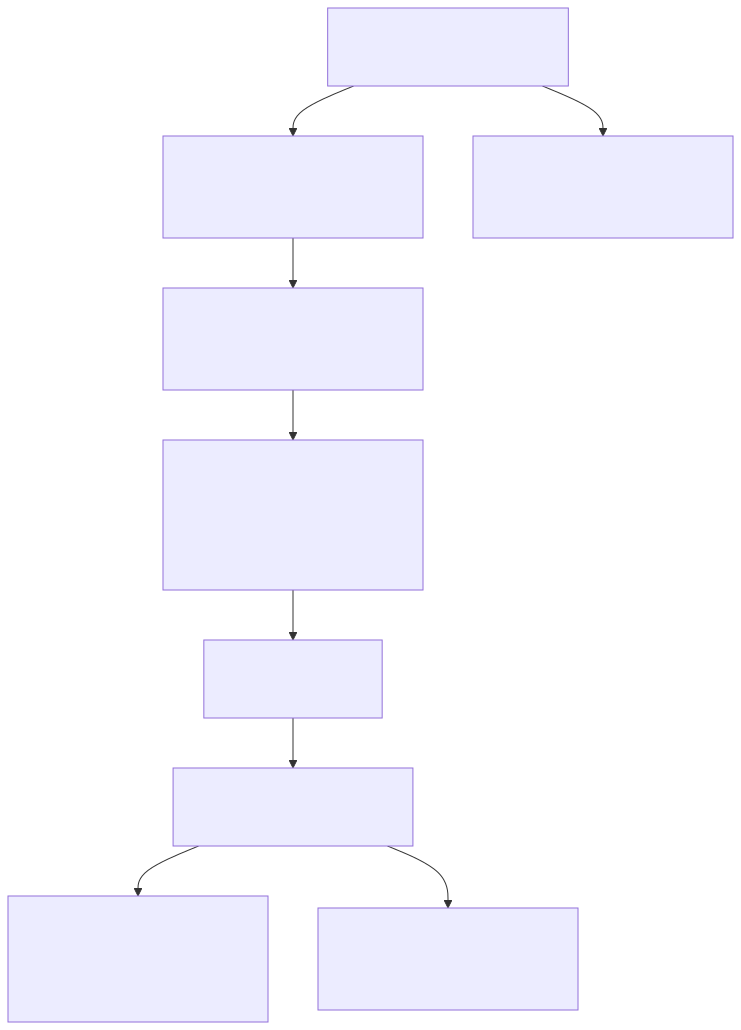
\includegraphics[width=\maxwidth,keepaspectratio,alt={Mermaid Diagram 1}]{0010-automatic-path-discovery/mermaid_1.png}}
\caption{Mermaid Diagram 1}
\end{figure}

\emph{Fig. 1: Network topology for BFA-inspired network probing}

The probing traffic from node A would follow the BFA pattern of
establishing telemetry from the immediate vicinity of A using 1-hop
probing traffic:

\begin{codebubbleenv}
A -> B -> A
A -> C -> A
A -> D -> A
\end{codebubbleenv}

Once the immediate vicinity is probed and a basic topology map is
established, a larger share of the probing traffic SHOULD transition to
using the depth-first algorithm, phasing the BFA into a smaller
proportion of overall probing activity.

\subparagraph{4.2.1.2 Depth-first algorithm
(DFA)}\label{depth-first-algorithm-dfa}

Depth-first search (DFS) is a graph traversal algorithm that explores as
far as possible along each branch before backtracking. In the context of
network probing, DFS MUST start at the probing node and explore each
branch of the graph deeply before moving to another branch.

DFS is particularly useful for pathfinding and exploring specific routes
through the network to assess end-to-end path viability.

This algorithm SHOULD be primarily implemented using \textbf{n-hop to
self} probes, where \codebubble{n > 1} and
\codebubble{n ≤ MAX\_HOPR\_SUPPORTED\_PATH\_LENGTH} (a network parameter
defined in
\href{../RFC-0004-hopr-packet-protocol/0004-hopr-packet-protocol.md}{RFC-0004}).
Each edge SHOULD be probed as soon as feasible, but not at the expense
of other edges in the topology (i.e., probing should be distributed
across the topology). The value of \codebubble{n} SHOULD be chosen
randomly to prevent predictable probing patterns, but MUST conform with
the minimum requirement for edge traversal (typically n ≥ 2 for
meaningful path diversity assessment).

Given a network topology around node A (Fig. 2):

\begin{figure}
\centering
\pandocbounded{\includegraphics[width=\maxwidth,keepaspectratio,alt={Mermaid Diagram 2}]{0010-automatic-path-discovery/mermaid_2.png}}
\caption{Mermaid Diagram 2}
\end{figure}

\emph{Fig. 2: Network topology for DFA-inspired network probing}

The probing traffic from node A would follow the DFA pattern of
establishing telemetry to the furthest interesting point in the network
using n-hop probing traffic with \codebubble{n} generated randomly
within the allowed range:

\begin{codebubbleenv}
A -> B -> F -> A
A -> C -> F -> E -> A
A -> B -> D -> A
\end{codebubbleenv}

These deep probes explore specific paths through the network and collect
end-to-end path metrics.

\subparagraph{4.2.1.3 BFA and DFA
interactions}\label{bfa-and-dfa-interactions}

Average values calculated over the differences of various observations
can be used to establish individual per-node properties. By combining
telemetry from breadth-first and depth-first probes, it is possible to
derive statistical information about individual nodes and edges in the
topology.

\textbf{Example}: Assume the following average path latencies are
observed:

\begin{codebubbleenv}
A -> B -> A = 421ms
A -> B -> F -> A = 545ms
\end{codebubbleenv}

From these measurements, it is possible to estimate the average latency
contribution of node F (and the edges involving F) as:

\begin{codebubbleenv}
(A -> B -> F -> A) - (A -> B -> A) = 545ms - 421ms = 124ms
\end{codebubbleenv}

This difference represents the additional latency introduced by
traversing through node F. Accounting for artificial mixer delays that
introduce additional anonymity, repeated observations of this value
averaged over longer time windows would provide an expected latency
contribution for node F. By aggregating such measurements across
multiple paths, implementations can build a statistical model of
individual node performance characteristics.

\paragraph{4.2.2 Evaluation mechanism}\label{evaluation-mechanism}

The evaluation mechanism processes probe results to assess path and node
viability. The mechanism SHOULD maintain short-term memory of recent
probe results and apply balanced scoring that equally rewards probe
successes and penalises probe failures. This approach ensures that
recent network conditions are given appropriate weight while preventing
both overly optimistic and overly pessimistic assessments.

Implementations MAY use various evaluation strategies, such as
exponentially weighted moving averages, sliding time windows, or
Bayesian estimation, provided they meet the requirement of balanced
success/failure treatment.

\paragraph{4.2.3 Retention and slashing
mechanism}\label{retention-and-slashing-mechanism}

Nodes MAY implement a slashing mechanism based on failed probes to
prevent using unreliable relay nodes in non-probing (production)
communication, thereby avoiding dropped messages and improving overall
communication reliability.

The slashing mechanism operates by temporarily or permanently removing
nodes or paths from the usable path pool based on probe failure
patterns. Implementations SHOULD consider:

\begin{itemize}
\tightlist
\item
  \textbf{Failure threshold}: The number or percentage of consecutive or
  recent failed probes that trigger slashing.
\item
  \textbf{Slashing duration}: Whether nodes are removed permanently or
  temporarily \\(with exponential backoff for repeated failures).
\item
  \textbf{Recovery mechanism}: Conditions under which previously slashed
  nodes can be re-evaluated and restored to the usable pool.
\end{itemize}

Slashing decisions SHOULD be made locally by each node based on its own
probe observations, without coordination with other nodes.

\paragraph{4.2.4 Throughput
considerations}\label{throughput-considerations}

Paths SHOULD be selected and used by the discovery mechanism in a manner
that supports sustained throughput (i.e., the maximum achievable packet
rate). Path selection SHOULD consider:

\begin{itemize}
\tightlist
\item
  \textbf{Load balancing over paths}: Distribute traffic across multiple
  paths based on the minimum stake (channel balance) on each path,
  ensuring paths with higher capacity receive proportionally more
  traffic.
\item
  \textbf{Measured throughput}: Use actual throughput as observed in
  real traffic (not just probes) to refine path selection and avoid
  paths that perform poorly under load.
\end{itemize}

These considerations ensure that path discovery supports not only path
viability assessment but also efficient utilisation of available network
capacity.

\subsubsection{4.3 Telemetry}\label{telemetry}

Telemetry refers to the data and metadata collected by the probing
mechanism about traversed transport paths. Telemetry enables nodes to
assess path quality, detect failures, and make informed path selection
decisions. This section defines the types of telemetry collected and
their purposes.

\paragraph{4.3.1 Next-hop telemetry}\label{next-hop-telemetry}

Next-hop telemetry, also referred to as per-path telemetry (PPT), MUST
be collected for each direct peer connection. This telemetry SHOULD be
used to inform channel opening and closing strategies that optimise
first-hop connections from the current node.

The PPT SHOULD provide basic evaluation of the transport channel, both
in the presence and absence of an open on-chain payment channel. At a
minimum, the PPT MUST provide the following observations for each 0-hop
connection (as specified in
\href{../RFC-0004-hopr-packet-protocol/0004-hopr-packet-protocol.md}{RFC-0004}):

\begin{enumerate}
\def\labelenumi{\arabic{enumi}.}
\item
  \textbf{Latency}: Duration between sending a message and receiving the
  corresponding acknowledgement. This measures round-trip time to the
  immediate peer.
\item
  \textbf{Packet drop rate}: Track the ratio of missing acknowledgements
  to expected acknowledgements for messages sent on the channel. This
  indicates the reliability of the transport connection.
\end{enumerate}

The PPT MAY be utilised by other mechanisms as an information source,
such as channel management strategies that optimise the outgoing network
topology by opening channels to high-performance peers and closing
channels to unreliable peers.

\paragraph{4.3.2 Non-probing telemetry}\label{non-probing-telemetry}

Non-probing telemetry refers to telemetry collected from production
(non-probe) traffic. This telemetry MAY track the same metrics as
next-hop telemetry with the goal of adding more relevant channel
information for 0-hop connections.

Each outgoing message SHOULD be tracked for the same set of telemetry as
the PPT (latency, packet drop rate) on a per-message basis. This
provides real-world performance data that complements probe-based
observations and can reveal issues that only appear under actual traffic
load.

\paragraph{4.3.3 Probing telemetry}\label{probing-telemetry}

Probing telemetry refers to structured data embedded within probe
messages to facilitate path identification and performance measurement.
All multi-byte integer fields MUST be transmitted in network byte order
(big-endian) to ensure consistent interpretation across different
architectures.

The probing message payload contains the following fields:

\begin{itemize}
\item
  \textbf{Counter} (8 bytes, \codebubble{uint64}): An iterating counter
  used to verify the mixing property over a path and detect packet
  reordering or duplication. The counter increments for each probe sent.
\item
  \textbf{Path ID} (8 bytes, \codebubble{uint64}): A unique identifier
  for a single specific path in the graph, enabling attribution of probe
  results to the correct path.
\item
  \textbf{Timestamp} (8 bytes, 64-bit
  \codebubble{UNIX time in nanoseconds}): The timestamp of packet
  creation, used for end-to-end latency observations. The timestamp is
  recorded when the probe is generated and compared against the received
  timestamp upon loopback completion.
\end{itemize}

\textbf{Wire format:}

\begin{codebubbleenv}
+-------------+------------+------------+
|   Counter   |   PathId   |  Timestamp |
|     8B      |     8B     |     8B     |
+-------------+------------+------------+
\end{codebubbleenv}

The total probing message payload size is 24 bytes.

\subsubsection{4.4 Component placement}\label{component-placement}

The network probing functionality, with the exception of the next-hop
telemetry (PPT) mechanism, MUST be implemented using HOPR loopback
communication to preserve anonymity and prevent relay nodes from
distinguishing probe traffic from production traffic.

\clearpage

\textbf{Implementation requirements:}

\begin{itemize}
\item
  \textbf{Remove channel graph quality}: The concept of channel graph
  quality based on network observations SHALL be removed from
  implementations. Only on-chain channel information (stake, balance,
  status) SHALL be retained for path viability determination.
\item
  \textbf{Continuous probe generation}: Implementations MUST provide
  processes to generate a low-rate continuous stream of network path
  probes to maintain up-to-date topology information.
\item
  \textbf{Session-specific paths}: Implementations MUST generate
  session-specific paths for session path selection to provide cover
  traffic and obfuscate the real communication patterns (see
  \href{../RFC-0008-session-protocol/0008-session-protocol.md}{RFC-0008}).
\item
  \textbf{Path graph system}: A new path graph system SHALL be derived
  from probe results, representing discovered topology and path quality
  metrics.
\item
  \textbf{Path caching}: Paths SHALL be cached for a configurable
  minimum time window to amortise the cost of path discovery and reduce
  probe frequency.
\item
  \textbf{Session metrics incorporation}: Session-level telemetry SHALL
  incorporate:

  \begin{itemize}
  \tightlist
  \item
    Session-level performance metrics (throughput, latency, packet loss)
  \item
    Session-specific path probing data to refine path selection during
    active sessions
  \item
    Session-derived cover traffic for exploratory network traversal
    without dedicated probe overhead
  \end{itemize}
\end{itemize}

\subsection{5. Design considerations}\label{design-considerations}

The automatic path discovery mechanism is designed to enable each sender
to:

\begin{enumerate}
\def\labelenumi{\arabic{enumi}.}
\item
  \textbf{Identify sufficient network nodes}: Discover a sufficiently
  large number of network nodes to ensure privacy through path pool
  diversity. A larger discovered topology enables greater path
  randomisation and reduces the risk of traffic analysis.
\item
  \textbf{Detect problematic nodes}: Identify unstable, malicious, or
  adversarial nodes through probe failure patterns and exclude them from
  path selection.
\item
  \textbf{Estimate QoS metrics}: Establish basic propagation metrics for
  quality-of-service (QoS) estimation, including latency, throughput,
  and reliability.
\end{enumerate}

With these capabilities, the sender can construct a functional
representation of the network topology, state, and constraints, enabling
optimal selection and exclusion of message propagation paths.

\textbf{Key design principles:}

\begin{itemize}
\item
  \textbf{Indistinguishability}: Multi-hop probing traffic and
  measurement packets MUST be indistinguishable from ordinary traffic to
  ensure accurate recording of network node propagation characteristics.
  If relay nodes could distinguish probes from production traffic, they
  might handle them differently (e.g., prioritise or deprioritise
  probes), leading to inaccurate measurements.
\item
  \textbf{Adaptive mechanisms}: Due to the dynamic nature of
  decentralised peer-to-peer networks, senders SHOULD employ adaptive
  mechanisms for establishing and maintaining topological awareness.
  Static path selection would quickly become outdated as nodes join,
  leave, or change behaviour.
\item
  \textbf{Continuous probing}: For both unidirectional and bidirectional
  communication to adapt to changing network conditions, senders MUST
  actively probe the network in a continuous manner, with probe
  frequency balanced against economic feasibility.
\item
  \textbf{Economic feasibility}: Measurement traffic SHOULD adhere to
  economic feasibility constraints, i.e., it SHOULD be proportional to
  actual message traffic. Excessive probing wastes network resources and
  incurs unnecessary costs. Probe traffic MAY be incorporated as part of
  cover traffic (see
  \href{../RFC-0008-session-protocol/0008-session-protocol.md}{RFC-0008})
  to serve dual purposes.
\item
  \textbf{No telemetry sharing}: Any measurements obtained from probing
  traffic SHOULD be node-specific and MUST NOT be subject to data or
  topology exchange with other nodes. Sharing telemetry could compromise
  anonymity by revealing which nodes are being probed and what paths are
  being considered.
\end{itemize}

\textbf{Telemetry requirements:}

The collected telemetry for measured paths:

\begin{itemize}
\tightlist
\item
  MUST contain path passability data indicating whether paths are
  traversable by single or multiple messages.
\item
  MAY include additional information such as latency, packet loss rate,
  and throughput, transmitted as message content in the probing payload.
\end{itemize}

\clearpage

\textbf{Direct peer probing:}

By designing probing traffic to be indistinguishable from actual message
propagation in the mixnet, direct verification of immediate peer
properties becomes infeasible. For this purpose, a separate mechanism
(next-hop telemetry, Section 4.3.1) exists that operates outside the
anonymity requirement.

The 0-hop and 1-hop probing mechanisms MAY NOT fully comply with the
anonymity requirement, since they:

\begin{enumerate}
\def\labelenumi{\arabic{enumi}.}
\tightlist
\item
  Mimic the 0-hop session
  (\href{../RFC-0008-session-protocol/0008-session-protocol.md}{RFC-0008}),
  which does not benefit from multi-hop relaying mechanisms and may
  reveal the probing node to the immediate peer.
\item
  Could be used as a first layer for relay nodes to discover viable
  candidates for future channel openings, which is acceptable as it does
  not compromise sender anonymity in multi-hop paths.
\end{enumerate}

The network probing mechanism SHALL utilise graph-based algorithms
(breadth-first and depth-first) to efficiently discover and maintain
network topology information while managing computational and economic
costs.

\subsection{6. Compatibility}\label{compatibility}

The automatic path discovery mechanism is a local node feature that
affects only the implementing node. Changes to path discovery algorithms
or telemetry collection MAY be modified without impacting overall
network operation, as long as the node continues to generate valid HOPR
packets and respects protocol semantics.

The network probing mechanism is compatible with the loopback session
mechanism defined in
\href{../RFC-0008-session-protocol/0008-session-protocol.md}{RFC-0008},
allowing probes to leverage session infrastructure when available.

\subsection{7. Security considerations}\label{security-considerations}

The probing traffic consumes both physical resources (bandwidth,
compute) and economic value (payment channel balances) at various levels
of the HOPR protocol stack. This resource consumption introduces several
security considerations:

\begin{enumerate}
\def\labelenumi{\arabic{enumi}.}
\item
  \textbf{Resource depletion attacks}: In highly volatile networks,
  adversarial behaviour may cause excessive resource expenditure through
  probe failures or artificial network instability. Attackers could
  deliberately fail probes to force nodes to increase probe frequency,
  potentially enabling resource depletion attacks. Implementations
  SHOULD implement rate limiting and adaptive probe frequency to
  mitigate this risk.
\item
  \textbf{Denial-of-service via PPT}: The next-hop telemetry (PPT)
  mechanism, which operates at 0-hop without full anonymity protection,
  MAY serve as an attack vector for denial-of-service (DoS) attempts.
  Attackers could flood a node with 0-hop telemetry requests to exhaust
  resources. Implementations SHOULD apply rate limiting to PPT requests.
\item
  \textbf{Traffic analysis}: Although probes are designed to be
  indistinguishable from production traffic, statistical analysis of
  traffic patterns might reveal probing behaviour if probe generation
  follows predictable patterns. Implementations SHOULD randomise probe
  timing and path selection to prevent traffic analysis.
\item
  \textbf{Mitigation strategies}: Nodes MAY implement any reasonable
  security risk mitigation strategy, including but not limited to:

  \begin{itemize}
  \tightlist
  \item
    Rate limiting probe generation and reception
  \item
    Adaptive probe frequency based on network conditions
  \item
    Slashing mechanisms to exclude misbehaving nodes
  \item
    Resource quotas for probe traffic
  \end{itemize}
\end{enumerate}

\subsection{8. Drawbacks}\label{drawbacks}

The network probing mechanism has several inherent limitations:

\begin{enumerate}
\def\labelenumi{\arabic{enumi}.}
\item
  \textbf{Resource consumption}: Probing activity consumes network
  bandwidth, computational resources, and payment channel balances.
  Implementations MUST carefully balance probing and data transmission
  activities to maintain reasonable resource utilisation ratios.
  Excessive probing wastes resources; insufficient probing leads to
  outdated topology information.
\item
  \textbf{Scalability limitations}: Complete real-time probing of large
  networks is computationally prohibitive. As network size increases,
  the number of possible paths grows combinatorially, making exhaustive
  probing infeasible. Algorithms SHOULD operate within bounded
  subnetworks where they can provide reasonable network visibility
  guarantees within acceptable resource constraints.
\item
  \textbf{Bootstrap requirements}: Prior knowledge of target nodes
  (e.g., through external discovery mechanisms or bootstrap node lists)
  is advantageous to minimise initialisation time before establishing a
  sufficient network view for informed path selection. Nodes joining a
  network without any peer knowledge face a cold-start problem.
\end{enumerate}

\subsection{9. Alternatives}\label{alternatives}

No known alternative mechanisms exist that simultaneously: - Preserve
sender anonymity by preventing relay nodes from distinguishing probes -
Maintain trustless properties without requiring nodes to share topology
information - Consolidate probing control under the communication source
to enable informed path selection

Alternative approaches such as centralised topology databases or
distributed topology sharing protocols would compromise either anonymity
or trustlessness, making them unsuitable for the HOPR protocol's threat
model.

\subsection{10. Unresolved questions}\label{unresolved-questions}

None.

\subsection{11. Future work}\label{future-work}

Future development of the automatic path discovery mechanism SHOULD
focus on the following areas:

\begin{enumerate}
\def\labelenumi{\arabic{enumi}.}
\item
  \textbf{Extended telemetry collection}: Improve the ability to collect
  additional network metrics by extending the data payload transmitted
  along the loopback path. Additional metrics might include jitter,
  packet reordering, or relay node load indicators.
\item
  \textbf{Advanced path generation strategies}: Develop new
  path-generating strategies that enable statistical inference of
  information from path section overlaps. For example, using matrix
  completion techniques or Bayesian inference to estimate properties of
  un-probed edges from probed path combinations.
\item
  \textbf{Enhanced evaluation mechanisms}: Improve metric evaluation
  mechanisms with more sophisticated scoring functions, machine
  learning-based anomaly detection, or adaptive weighting schemes that
  respond to network conditions.
\item
  \textbf{Formal slashing logic}: Define a formal slashing mechanism
  with equation-based logic that specifies precise conditions for node
  removal, recovery, and reputation scoring.
\end{enumerate}

\subsection{12. References}\label{references}

None.
